\documentclass[letterpaper,10pt]{article}
\usepackage{graphicx}
\usepackage{amsmath,amssymb,array,calc,epsfig,rotating,bm}
\usepackage[sort]{cite}
\usepackage{psfrag,verbatim}
\usepackage{mathtools}

\def\code#1{\texttt{#1}}

%opening
\title{Triangulating polygons}
\author{Anton van Niekerk}

\begin{document}

\maketitle

\begin{abstract}
I describe a program designed to  colour the vertices such that a target number of triangles in the graph are neutrally coloured.
This program is then applied to a particular problem.
\end{abstract}

\section{Summary of problem and solution}
\subsection{Problem}
The problem is to colour the uncoloured vertices in figure \ref{problemfig} so that there are exactly $2$ neutral triangles in the coloured graph. 

\begin{figure}
\begin{center}
  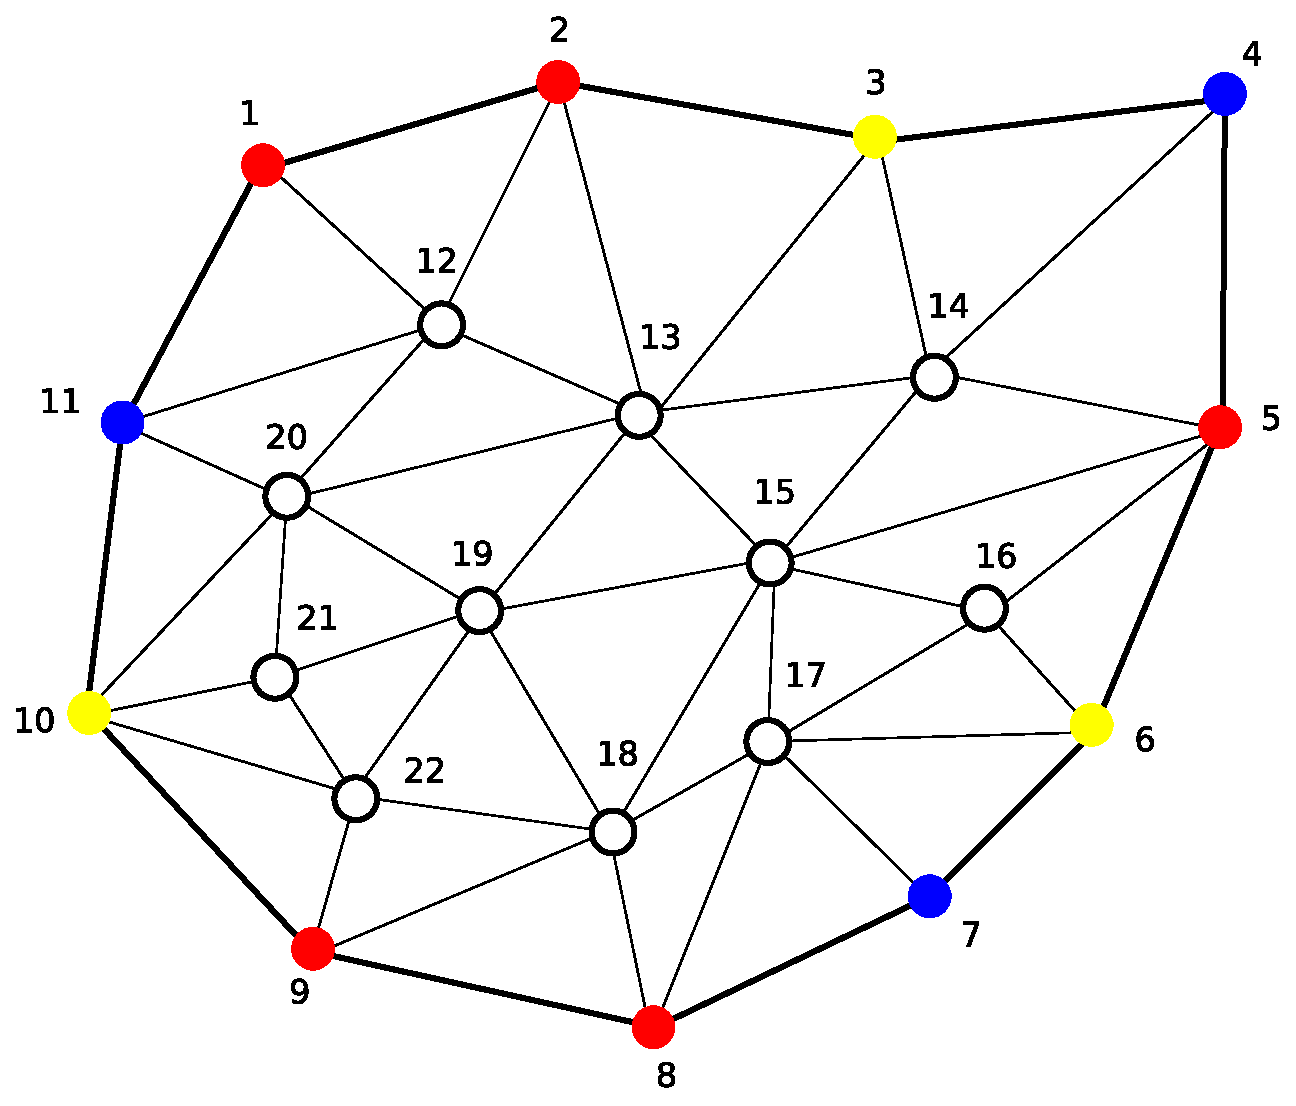
\includegraphics[width=3in]{tripoly.eps}
\end{center}
  \caption{
The graph for the coding problem, with the vertices numbered as implemented in Java.} \label{problemfig}
\end{figure}
\subsection{Algorithm}
There are $11$ uncoloured vertices, each being able to be coloured $3$ different colours.  That means that there are $11^3 = 1331$ possible colourings 
of the graph.  There are also $31$ different triangles in the graph, meaning that a brute force algorithm that checks each triangle for neutrality 
in every possible colouring of the graph must check  
\begin{equation} \label{eq1}
 31\times11^3 = 41216
\end{equation}
 different triangles for neutrality if no solution exists.

The algorithm I came up with for colouring the graph is instead to colour the vertices one by one in the sequence defined by the numbering in 
the figure as follows (see also comments in the code itself for where each step occurs):
\begin{enumerate}
 \item The current vertex is assigned a colour (starting with the first uncoloured vertex) from the list $\{\textrm{red},\,\textrm{blue},\,\textrm{yellow}\}$.  
 \item To reduce the number of triangles to be checked for neutrality, 
 only the triangles with the current vertex as a corner are checked for neutrality, 
 with the total new neutral triangles added to the running total.
 \item If the total number of neutral triangles don't exceed the target 
 ($2$ in this case), then the next vertex will be coloured.  
  \item If the target number of neutral triangles is exceeded, then the current vertex will be assigned the next colour from the list.
  \item If all colours are used up for the present vertex without achieving the target, then the current vertex will be made colourless,  
and the previous vertex will be assigned the next colour from the list.
  \item If the final vertex is assigned a colour and the target is achieved, we break out of this algorithm and leave the graph coloured so that it 
  solves the problem.
  \item If all colours in the list are attempted for the first vertex without achieving the target, it means that all possible colourings for the 
  graph have been attempted, and there is no solution.  We therefore return the graph uncoloured and return an error code.
\end{enumerate}
\subsection{Algorithm efficiency}
Although I came up with this algorithm on my own, it was inspired at least in part by the tree-based searching algorithms as set out in 
\cite{inspiration}.  In fact, this algorithm can be viewed as following a path down a decision tree, where each branch represents the decision of 
whether to colour a particular vertex a certain colour.  The leaves of the tree then represent a particular colouring of the graph.  
If a node is reached, and the total number of neutral triangles exceed the target number, or we reach a leaf and the target is not met, 
then we go up the branch to the earliest ancestor node where the target is not yet exceeded, and follow the tree decision branches until the next 
violation of the target condition occurs, or the target is met.

Because this algorithm can be viewed as traversing a tree, in some sense the average behaviour is that it needs to check of order of the logarithm 
of the total number of total possible triangles as calculated in equation \ref{eq1}.  However, the true behaviour is somewhat more difficult to 
estimate, given that the algorithm can run up and down the branches of the tree multiple times.  What can be said is that if no solution exists, then in the worst case 
much fewer triangles than the number of equation \ref{eq1} need to be checked, 
since triangles that were checked at an ancestor node don't need to be checked again.  So in some sense, the worst case behaviour 
is also the logarithm of the number of triangles checked in the brute force algorithm.

\subsection{Answer to the triangulation coding problem}
\textbf{The answer is no}.  That is, my algorithm finds that there is no colouring of the vertices such that there are exactly $2$ neutral triangles.
The method I wrote to find the solution can be applied to any graph, for any goal, and finds that the targets for which the problem has a solution are 
\begin{equation}
 \{3,\,5,\,7,\,9,\,11,\,13,\,15,\,17,\,19,\,21\},
\end{equation}
as can be found out by running the code.

\subsection{Time spent on problem}

Including planning, coding, debugging and writing this readme file, I spent approximately 20 - 24 hours on this problem.

\section{Description of code}
\subsection{Installation and execution instructions}
This code is written in Java, and should be able to compile using version 5 or later.

To run in Eclipse, create a new Java project.  Make sure the 
compiler compliance is set to 1.5 or above.  Right-click on the 
src folder and create a new package with the name ``triangulationProblem'', then import the unzipped package folder included in the email into the package.  
The code should compile correctly.

The class that needs to be run to solve the problem 
is \code{NeutralTriangles}.  The class \code{UnitTest} has test methods that can be run as JUnit Tests.  I had to add JUnit4 to my build-path 
for \code{UnitTest} to work without error.

\subsection{Classes and methods}
The code is structured so that it may form part of a larger project, or extended to do many other possible graph computations.  
As written it can already be applied to colour an arbitrary connected  graph, with the aim of achieving some \textit{goal} number of neutral triangles.
The classes, most important methods, and their descriptions are given below:

\begin{itemize}
 \item \code{GraphProperties}:  Contains the \textit{enum} \code{VertexColour} with the three colours a vertex can have.  
 \code{VertexColour} contains the methods \code{getColourName} for returning the string value of a colour, and \code{getColour} for returning 
 the \textit{enum} element corresponding to a string.
 
 \item \code{Vertex}: Has the constructors for creating a new instance of a vertex in the graph.  A vertex can have the properties \textit{name}, 
 which is an integer (as in figure \ref{problemfig}) and \textit{colour}, which is one of the elements of \code{VertexColour}, or can be null.  
 It also has getters and setters for these properties.  This class overrides \code{Object}'s \code{equals} method to check equality of a vertex 
 based on its \textit{name} only, as that is all that is required in this program.
 
 \item \code{PolygonGraph}: Is an instance of the graph and its properties.  It contains three separate hashmaps with values being the vertices of the graph, 
 arrays of vertices that are the nearest neighbours of each vertex (i.e., are connected with an edge to that vertex), and arrays of the triangles 
 that a vertex forms part of (each triangle being an array with three instances of \code{Vertex}).  
 The key for each of these hashmaps is the integer assigned to the vertex in the diagram (see figure \ref{problemfig}).
 
 The graph is not built with a single constructor call, but rather is constructed by repeatedly calling the method \code{setNrstNbrs}, which takes 
 two \code{int}s representing the \textit{name}s of vertices in the graph.   This method represents two vertices being joined by an edge in the graph.
 If one or both of the vertices are new, it is added to the hashmap \textit{vertices}.  Both vertices are added to each other's nearest neighbours 
 in the hashmap \textit{nearestNeighbours}.  If there is a third vertex that is the nearest neighbour to both vertices, they form a triangle, and 
 an array with all three vertices is added to the hashmap \textit{triangles} with the \textit{name} of \underline{each} vertex used as a key. 
 
 Other methods in this class are getters and setters allowing one to get and set a vertex's \textit{colour} and \textit{name} without 
 needing to directly access the vertex, as well as an array with its nearest neighbours.
 
 \item \code{NeutralTriangles}: Contains the static methods that are designed to answer the specific class of questions posed by the problem.
 \code{isTriangleNeutral} determines if a triangle's vertices have all three colours and is therefore neutral.  \code{countNeutralTriangles} uses 
 \code{isTriangleNeutral} to count the number of neutral triangles that a given vertex belongs to.  
 
 \code{colourGraph} takes as input a graph, 
 the integer \textit{name} of the first uncoloured vertex by the chosen numbering convention, the target number of neutral triangles and the current 
 number according to the colouring of the graph.  It then colours the graph according to the target, if possible, as described in more detail in 
 section 1.
 
 \code{drivewyzeGraphSetup} sets up the specific graph for the triangulation coding problem, as shown in figure \ref{problemfig}.  Finally 
the \code{main} method runs the program and outputs the solution, as well as all target numbers of 
neutral triangles that are possible.

\item \code{UnitTest}:  This class contains  test methods testing the functionality of the program.  It also has some static methods that create 
the small graphs shown in figure \ref{test1} to test \code{colourGraph}.

\end{itemize}


\begin{figure}
\begin{center}
  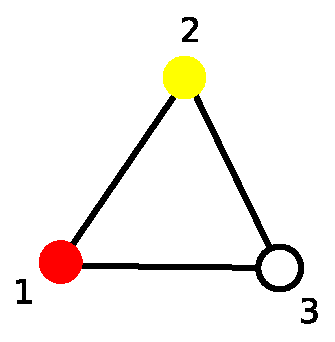
\includegraphics[width=1in]{triangle.eps}
  \qquad
  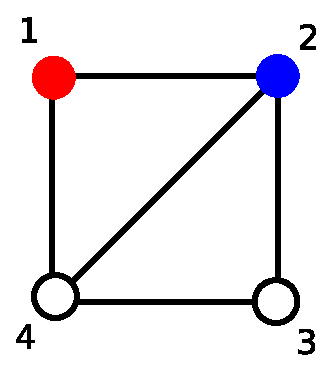
\includegraphics[width=1in]{square1.eps}
  \qquad
  \includegraphics[width=1in]{square2.eps}  
\end{center}
  \caption{
The graphs used for testing the algorithm and its failure in the unit test.} \label{test1}
\end{figure}


\section{Concluding remarks}
\subsection{Things I would change on a second attempt}
There are a few potential improvements that could be made:
\begin{enumerate}
 \item I was not very careful with public and private methods.  If I had more time, I would fix that.
 \item I was also not too careful with using \code{Integer} vs. \code{int} in my code.
 \item Currently the graph is initialized in the code itself.  Ideally the nearest neighbour relations between vertices, as well as their colours 
 would be fed in with a CSV file.  There would then be a method that could take that input and generate the graph and all its properties.
 \item Triangles are currently just \code{ArrayList}s containing 3 \code{Vertex} objects.  It would be more appropriate if there was a class 
 \code{Triangle} to contain the vertices.
 \item The class \code{PolygonGraph} contains three hashmaps, using the integer \textit{name} of the vertex as a key.  Ideally, the key to these 
 hashmaps would be the \code{Vertex} object itself, rather than the integer we have assigned to it.
 \item The method \code{colourGraph} returns the integer value of $0$ when the goal of $0$ neutral triangles cannot be achieved, rather than 
 the expected value of $-1$.  This is an error that should be fixed.
\end{enumerate}


\subsection{Acknowledgements}
The code was written in Eclipse Platform version 3.8.1.  The diagrams in this readme was created using Inkscape 0.48, and the readme itself was created 
in \LaTeX.


I referred to several sources while writing the code.  For unit testing I used the top answer in \cite{unittesting}. For writing, compiling and debugging Java,
I referred to \cite{basicjava}.  For creating the figures in the readme, I referred to \cite{inkscape}.  \LaTeX\,related questions were 
referred to in \cite{tex}.



\begin{thebibliography}{99}
\bibitem{inspiration}
Arne Storjohann, University of Waterloo CS240 Lecture Notes Based on lecture notes by R. Dorrigiv and D. Roche, 2013.
\bibitem{unittesting}
stackoverflow.com/questions/8751553/how-to-write-a-unit-test
\bibitem{basicjava}
docs.oracle.com/javase/tutorial/java/javaOO/constructors.html\\
docs.oracle.com/javase/tutorial/java/javaOO/enum.html\\
stackoverflow.com/questions/3811012/can-not-compile-enums-in-eclipse\\
stackoverflow.com/questions/2642589/how-does-a-arraylists-contains-method-evaluate-objects\\
stackoverflow.com/questions/18946657/cannot-instantiate-the-type-set
\bibitem{inkscape}
inkscape.org/en/doc/tutorials/shapes/tutorial-shapes.en.html\\
tavmjong.free.fr/INKSCAPE/MANUAL/html/Z-Order.html
\bibitem{tex}
tex.stackexchange.com/questions/74353/what-commands-are-there-for-horizontal-spacing\\
tex.stackexchange.com/questions/36030/how-to-make-a-single-word-look-as-some-code


\end{thebibliography}




\end{document}
